\section{Gleichstromsteller (Chopper)}

Ein Gleichstromsteller wandelt eine konstante Gleichspannung $U_{DC}$ in eine
\textbf{stufenlos einstellbare Gleichspannung} $u_d$ durch schnelles Ein- und Ausschalten
eines Halbleiterschalters.

Typische Anwendungen:
\begin{itemize}
\item Drehzahlregelung von Gleichstrommaschinen,
\item Stromregelung in Antrieben,
\item DC-Zwischenkreise in Umrichtern.
\end{itemize}

Die Stellgrösse ist der \textbf{Tastgrad}:
\[
\boxed{d = \frac{t_{\mathrm{on}}}{T_s}}, 
\qquad T_s = \text{Schaltperiode}
\]

\subsection{Grundprinzip}

% --- bestehende Grafik: Grundschaltung Chopper ---
\begin{center}
    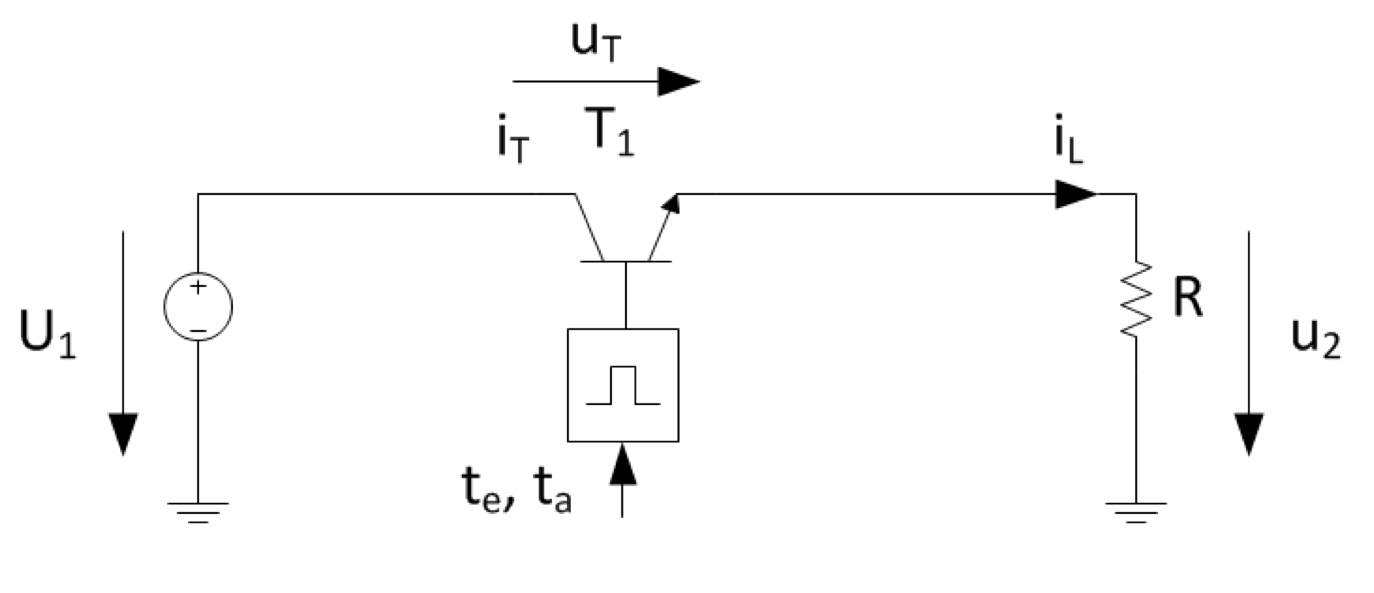
\includegraphics[width=0.85\linewidth]{images/Gleichstromsteller.png}
\end{center}

Während der Einschaltzeit $t_{\mathrm{on}}$ gilt:
\[
u_d(t) = U_{DC}
\]

Während der Ausschaltzeit $t_{\mathrm{off}}$ gilt (idealer Freilauf):
\[
u_d(t) = 0
\]

Mittelwert der Ausgangsspannung:
\[
\boxed{u_d = d \, U_{DC}}
\]

Dies ist identisch zum \textbf{Buck-Wandler} im kontinuierlichen Betrieb.

\subsection{Zeitbereich bei R--L-Last}

Bei R--L-Last gilt stückweise:

\paragraph{EIN-Phase}

\[
L \frac{di}{dt} + R i = U_{DC}
\]

Lösung:
\[
\boxed{
i(t) = \frac{U_{DC}}{R} + \left(i_{\min} - \frac{U_{DC}}{R}\right) e^{-t/\tau}
}, 
\qquad \tau = \frac{L}{R}
\]

\paragraph{AUS-Phase}

\[
L \frac{di}{dt} + R i = 0
\]

\[
\boxed{
i(t) = i_{\max} \, e^{-t/\tau}
}
\]

Periodenbedingung:
\[
\boxed{i_{\min} = i_{\max} \, e^{-T_a/\tau}}
\]

\subsection{Stromrippel und kontinuierlicher Betrieb}

Stromrippel:
\[
\boxed{
\Delta i = i_{\max} - i_{\min}
}
\]

Näherung für kleines R:
\[
\boxed{
\Delta i \approx \frac{(U_{DC} - u_d)\, d T_s}{L}
}
\]

Grenzinduktivität für kontinuierlichen Betrieb:
\[
\boxed{
L_{\min} = \frac{(1-d)R}{2 f_s}
}
\]

\begin{itemize}
\item $L > L_{\min}$ $\Rightarrow$ kontinuierlicher Betrieb (CCM),
\item $L < L_{\min}$ $\Rightarrow$ diskontinuierlicher Betrieb (DCM),
\item DCM $\Rightarrow$ Mittelwertformel $u_d = dU_{DC}$ gilt nicht mehr exakt.
\end{itemize}

\subsection{Einquadrantensteller (1Q)}

% --- bestehende Grafik: 1Q ---
\begin{center}
    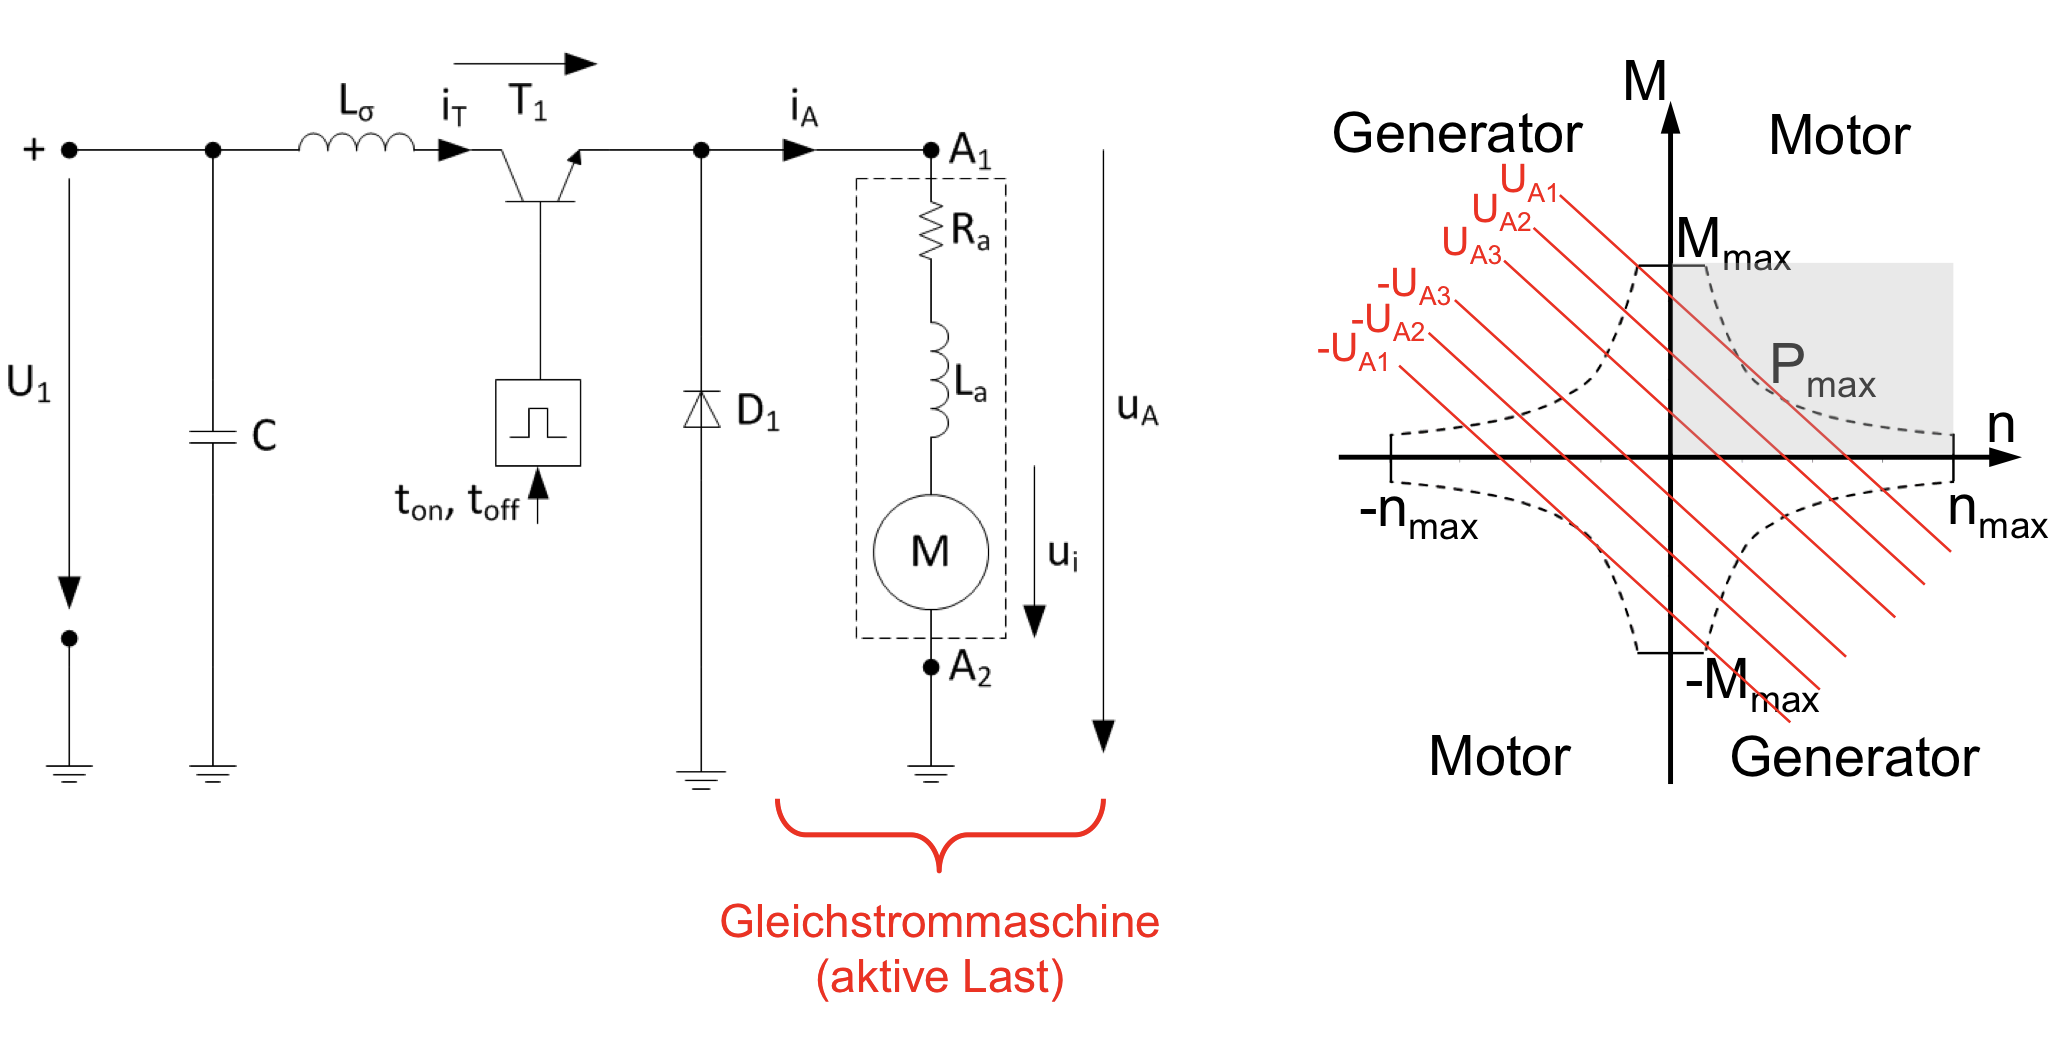
\includegraphics[width=0.85\linewidth]{images/Gleichstromsteller1Q.png}
\end{center}

Eigenschaften:
\begin{itemize}
\item $u_d \ge 0$, $i_d \ge 0$
\item Nur \textbf{Motorbetrieb vorwärts}
\end{itemize}

Spannungssteuerung:
\[
\boxed{u_d = d \, U_{DC}}
\]

Leistungsfluss:
\[
\boxed{P = u_d \, i_d > 0}
\]

Einsatz:
\begin{itemize}
\item Einfache Drehzahlregelung von Gleichstrommotoren,
\item Stromquellenbetrieb.
\end{itemize}

\subsection{Zweiquadrantensteller (2Q)}

% --- bestehende Grafik: 2Q ---
\begin{center}
    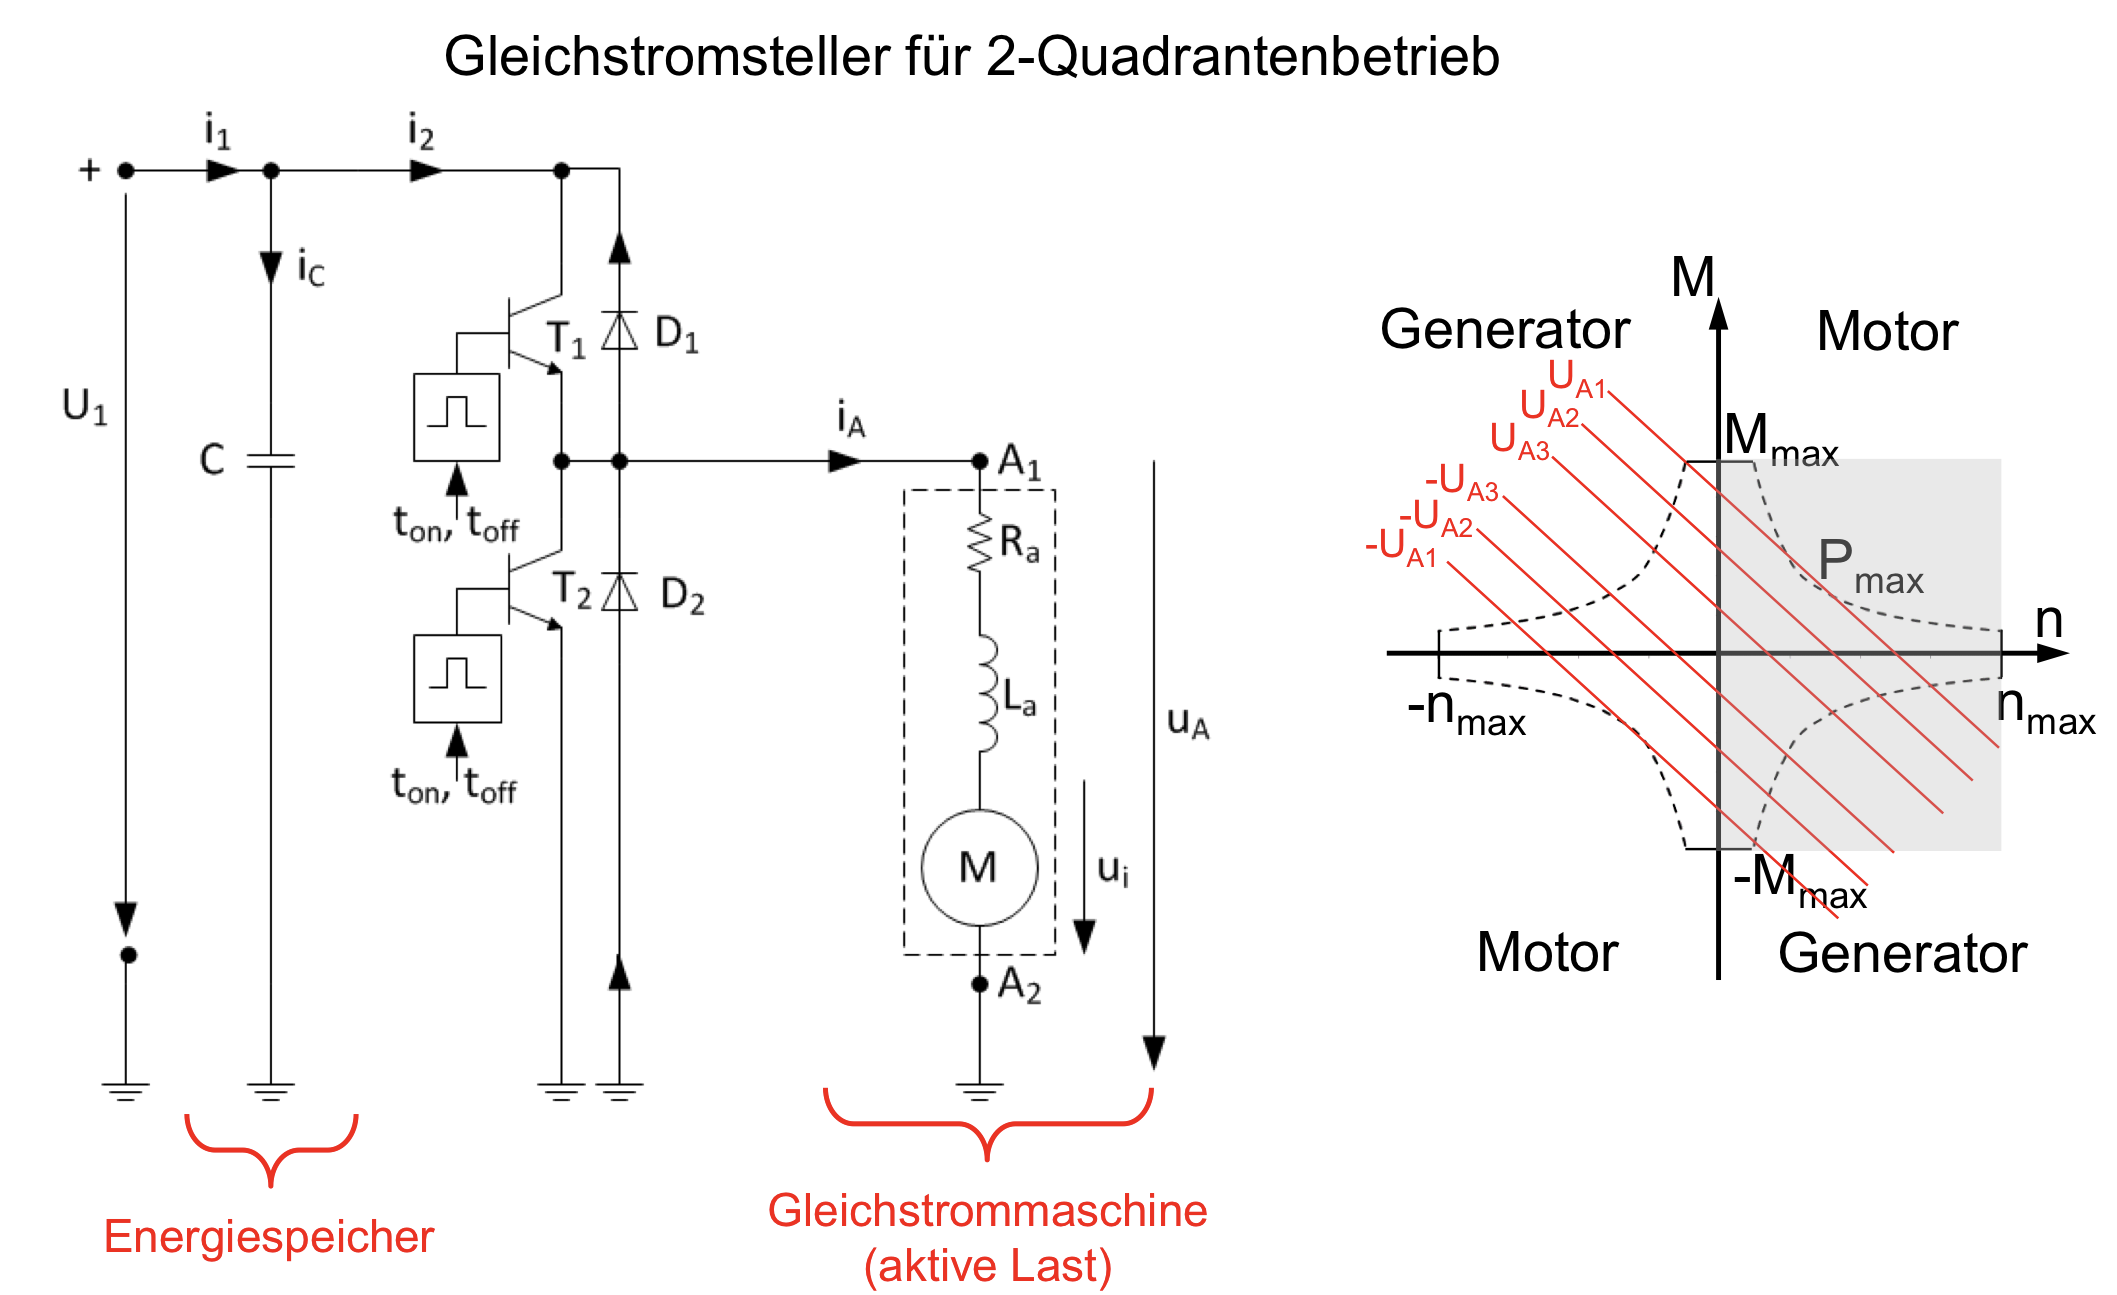
\includegraphics[width=0.85\linewidth]{images/Gleichstromsteller2Q.png}
\end{center}

Eigenschaften:
\begin{itemize}
\item $u_d \ge 0$
\item $i_d$ kann Vorzeichen wechseln
\item Motorbetrieb und \textbf{generatorischer Bremsbetrieb}
\end{itemize}

Beim Rekuperieren:
\[
\boxed{P = u_d \, i_d < 0}
\]

\begin{itemize}
\item Energie fliesst vom Motor zurück in die Quelle.
\item Typisch für elektrische Bremsung.
\end{itemize}

\subsection{Vierquadrantensteller (4Q)}

% --- bestehende Grafik: 4Q ---
\begin{center}
    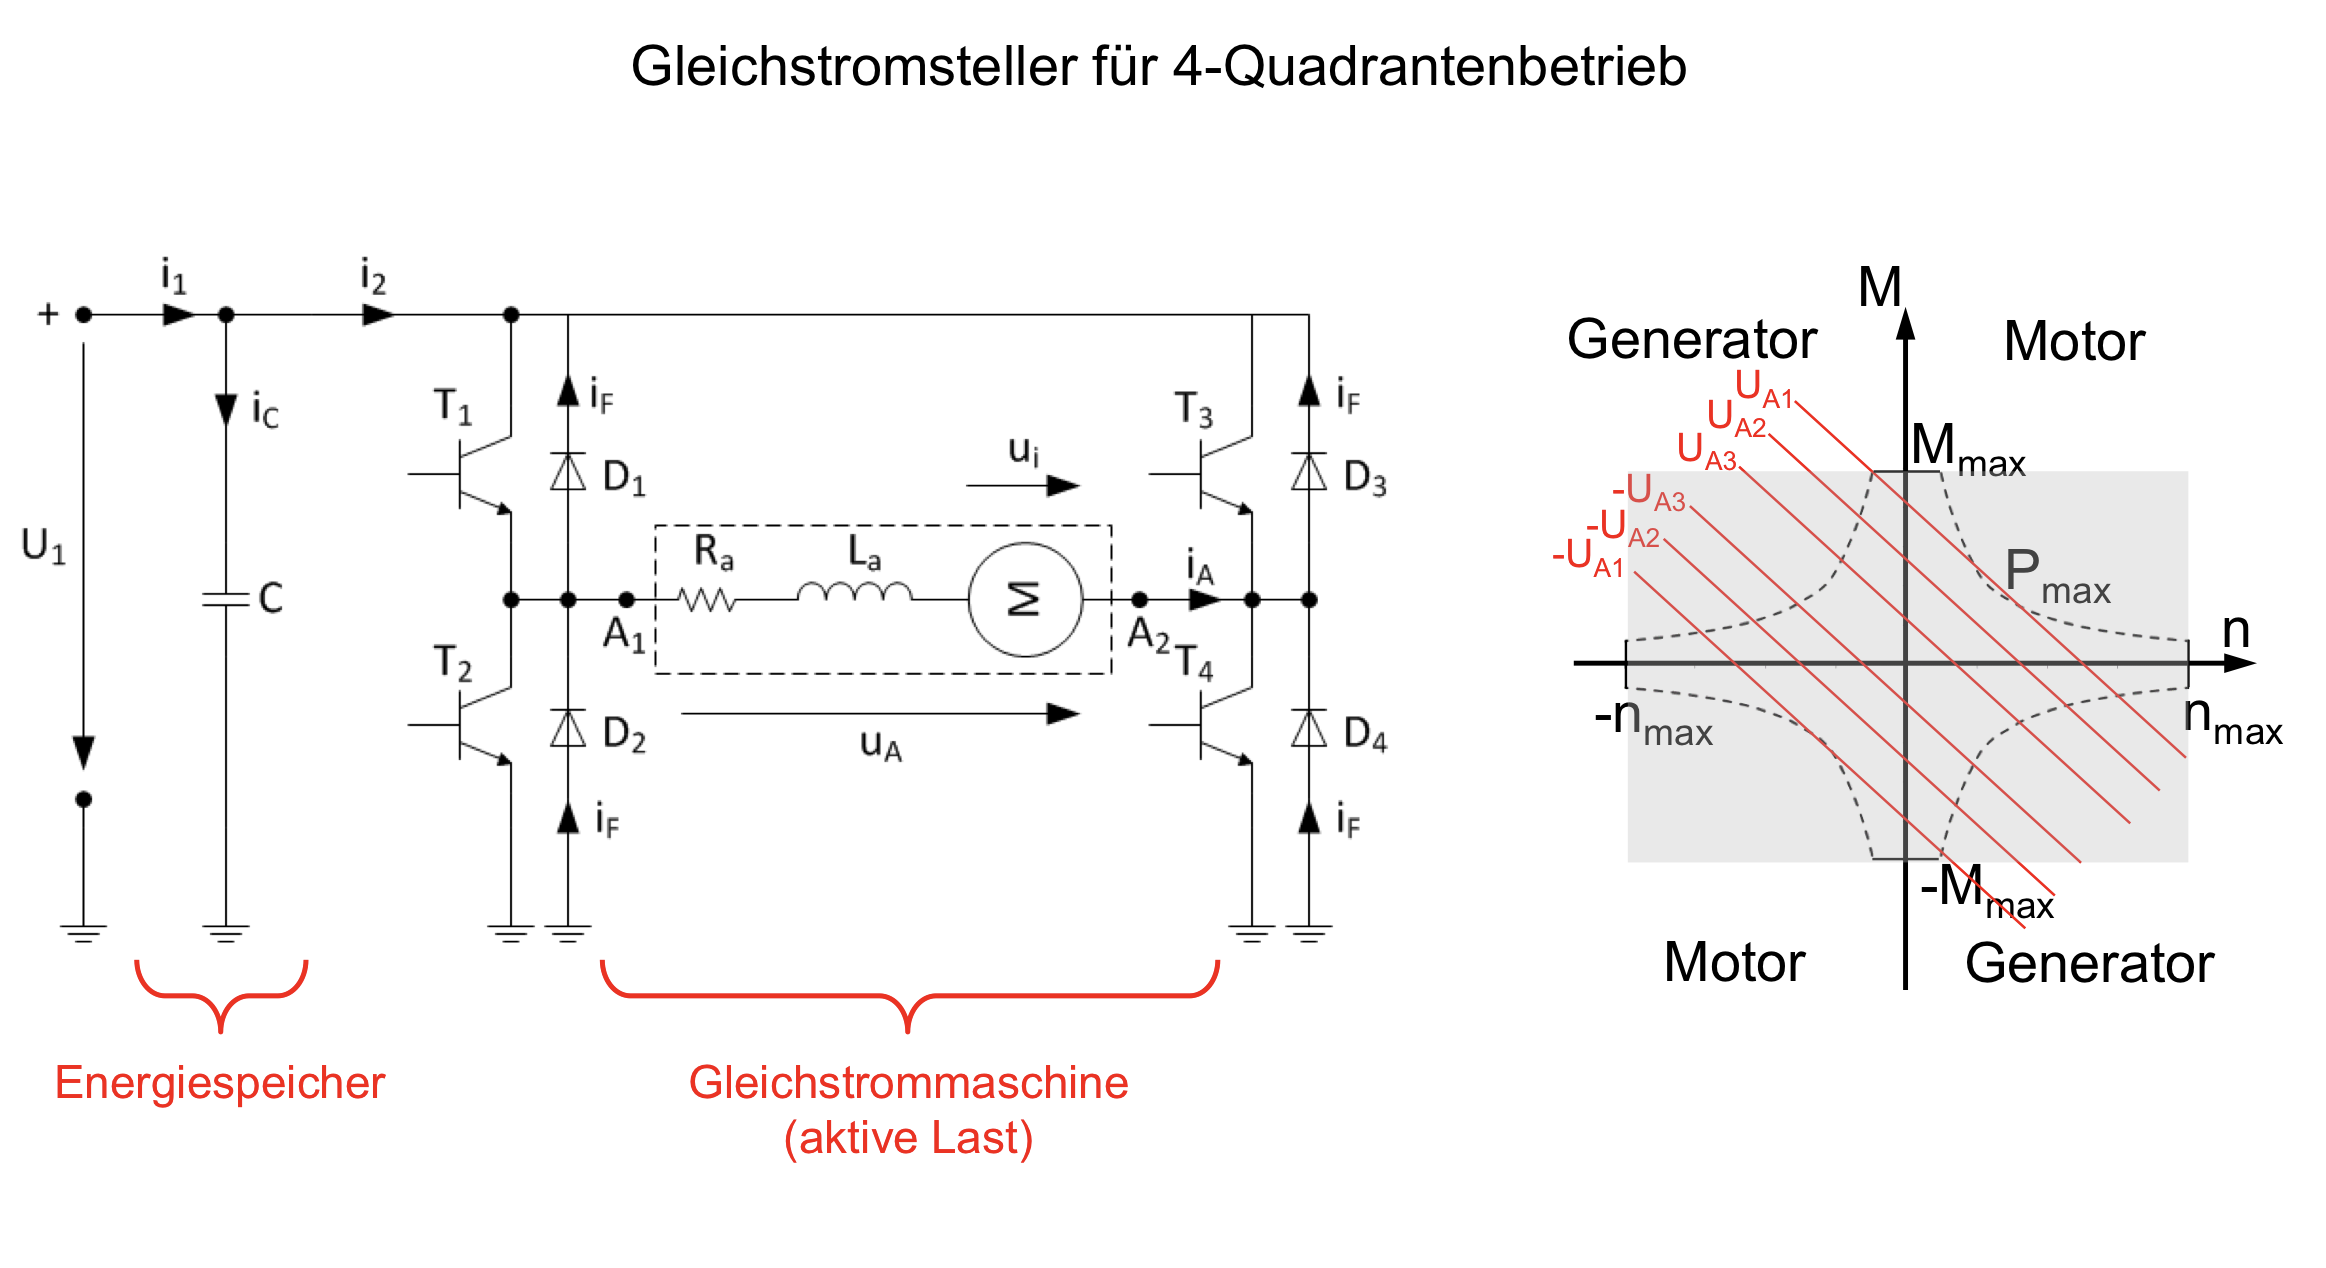
\includegraphics[width=0.85\linewidth]{images/Gleichstromsteller4Q.png}
\end{center}

Eigenschaften:
\begin{itemize}
\item $u_d$ vorzeichenwechselnd,
\item $i_d$ vorzeichenwechselnd,
\item Vollständiger Betrieb in allen Quadranten.
\end{itemize}

Quadranten:
\begin{itemize}
\item I: Motor vorwärts ($u>0,i>0$)
\item II: Generator vorwärts ($u<0,i>0$)
\item III: Motor rückwärts ($u<0,i<0$)
\item IV: Generator rückwärts ($u>0,i<0$)
\end{itemize}

Einsatz:
\begin{itemize}
\item Reversierantriebe,
\item Positionierantriebe,
\item Prüfstände.
\end{itemize}

\subsection{Bezug zur Gleichstrommaschine}

Für die DC-Maschine gilt:
\[
\boxed{u_d = R_a i_a + k\Phi \omega}
\]

Daraus:
\[
\boxed{\omega \approx \frac{u_d}{k\Phi} \quad \text{(bei kleiner Last)}}
\]

\begin{itemize}
\item $d\uparrow \Rightarrow u_d\uparrow \Rightarrow \omega\uparrow$
\item $d\downarrow \Rightarrow u_d\downarrow \Rightarrow \omega\downarrow$
\item Gleichstromsteller ist das \textbf{Standard-Stellglied} für DC-Antriebe.
\end{itemize}

\subsection{Vergleich zu Gleichrichtern}

\begin{itemize}
\item Gleichrichter: Spannung über Zündwinkel $\alpha$ gesteuert.
\item Gleichstromsteller: Spannung über Tastgrad $d$ gesteuert.
\item Gleichstromsteller arbeitet mit \textbf{hoher Schaltfrequenz}.
\item Gleichrichter arbeitet mit \textbf{Netzfrequenz}.
\end{itemize}

\subsection{Merksätze}

\begin{itemize}
\item Stellgrösse beim Gleichstromsteller ist der \textbf{Tastgrad $d$}.
\item $u_d = d U_{DC}$ gilt nur im \textbf{kontinuierlichen Betrieb}.
\item 1Q: nur Motorbetrieb vorwärts.
\item 2Q: Motor + generatorisches Bremsen.
\item 4Q: Motor und Generator in beiden Drehrichtungen.
\item Gleichstromsteller = Buck-Wandler für Antriebe.
\end{itemize}
